\documentclass[letterpaper,11pt,showproblems]{pset}
\usepackage{mmap} % make PDF files generated by pdfLaTeX both searchable and copy-able in acrobat reader and other compliant PDF viewers
\usepackage{graphicx}
\usepackage[plainpages=false,pdfpagelabels,unicode]{hyperref}

\usepackage{amsmath,amssymb,amsthm}

\newtheorem{thm}{Theorem}[section]
\newtheorem*{thm*}{Theorem}

\theoremstyle{definition} \newtheorem{defn}{Definition}[section]
\theoremstyle{definition} \newtheorem*{defn*}{Definition}

\newcommand{\thmref}[1]{Theorem~\ref{#1}}

\usepackage{xifthen}

\newcommand{\defeq}{\mathrel{\mathrel{\mathop:}\mkern -1.2mu=}}%\coloneqq}%\stackrel{\mathrm{df}}{=}}%{\ensuremath{:=}}%

\usepackage{pgf,tikz}
\usetikzlibrary{arrows}

\usepackage{array}
\usepackage{extarrows}

%\usepackage{caption}
%\captionsetup{justification=justified}
\usepackage{mathdots}

\psetnum{10}
\duedate{\TeX ed on \today}
\author{Jason Gross}
\classnumber{18.100C Recitation}
\classname{Real Analysis}
\professor{Peter Speh}
\begin{document}

\begin{center}\Large The Uncountability of the Reals \end{center}

\section{Audience: Child}
  \begin{center}
    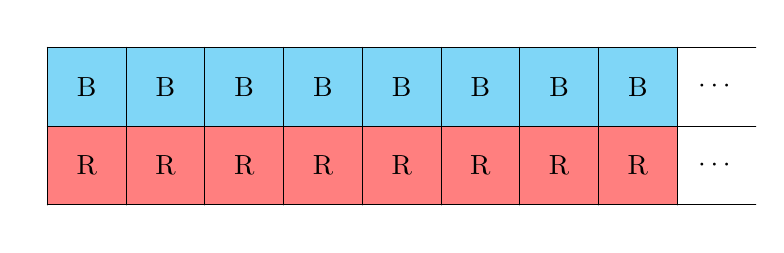
\begin{tikzpicture}[line cap=round,line join=round,>=triangle 45,x=1.0cm,y=1.0cm]
      \clip(-0.25,-1.25) rectangle (9,1.25);
      \foreach \x in {0,1,2,3,4,5,6,7}{
        \fill[cyan,opacity=0.5] (\x,1) -- (\x+1,1) -- (\x+1,0) -- (\x,0) -- cycle;
        \fill[red,opacity=0.5] (\x,-1) -- (\x+1,-1) -- (\x+1,0) -- (\x,0) -- cycle;
%         \foreach \y in {1,-1}{
%           \fill[white] (0.32+\x,0.68*\y) -- (0.68+\x,0.68*\y) -- (0.68+\x,0.32*\y) -- (0.32+\x,0.32*\y) -- cycle;
%         }
        \draw[color=black] (0.5+\x,0.5) node[anchor=center] {B};
        \draw[color=black] (0.5+\x,-0.5) node[anchor=center] {R};
        \draw (\x,1)-- (\x,-1);
      }
      \draw (8,1)-- (8,-1);

      \draw (8.5,0.5) node[anchor=center] {$\cdots$};
      \draw (8.5,-0.5) node[anchor=center] {$\cdots$};

      \draw (0,1) -- (9,1);
      \draw (0,0) -- (9,0);
      \draw[-,color=black] (0,-1) -- (9,-1);
    \end{tikzpicture}
  \end{center}
  Consider, as shown above, a sidewalk that goes on forever in one direction, which is made up of equal-sized square tiles.  The sidewalk is two squares across.  Consider a person who walks forever on it, obeying the following rule: Each step the person takes must be to one of the two tiles immediately in front of that person; no going backwards, no skipping tiles, no going sideways, no standing in place forever. The following is the beginning of one possible path:
  \begin{center}
    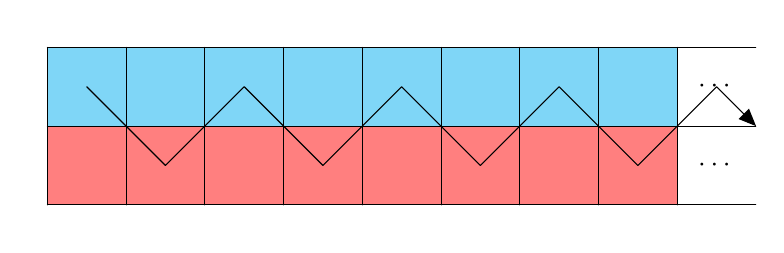
\begin{tikzpicture}[line cap=round,line join=round,>=triangle 45,x=1.0cm,y=1.0cm]
      \clip(-0.25,-1.25) rectangle (9,1.25);
      \foreach \x in {0,1,2,3,4,5,6,7}{
        \fill[cyan,opacity=0.5] (\x,1) -- (\x+1,1) -- (\x+1,0) -- (\x,0) -- cycle;
        \fill[red,opacity=0.5] (\x,-1) -- (\x+1,-1) -- (\x+1,0) -- (\x,0) -- cycle;
%         \foreach \y in {1,-1}{
%           \fill[white] (0.32+\x,0.68*\y) -- (0.68+\x,0.68*\y) -- (0.68+\x,0.32*\y) -- (0.32+\x,0.32*\y) -- cycle;
%         }
        \draw (\x,1)-- (\x,-1);
      }
      \draw (8,1)-- (8,-1);

      \draw (8.5,0.5) node[anchor=center] {$\cdots$};
      \draw (8.5,-0.5) node[anchor=center] {$\cdots$};

      \draw (0,1) -- (9,1);
      \draw (0,0) -- (9,0);
      \draw[-,color=black] (0,-1) -- (9,-1);
      \draw[->] (0.5,0.5) -- (1.5,-0.5) --
                (2.5,0.5) -- (3.5,-0.5) --
                (4.5,0.5) -- (5.5,-0.5) --
                (6.5,0.5) -- (7.5,-0.5) --
                (8.5,0.5) -- (9,0);
    \end{tikzpicture}
  \end{center}

  The statement that the reals are uncountable means that the number of different ways this person can walk forever, the number of paths this person can take, is strictly larger than the number of tiles that comprise the sidewalk.  ``Wait a minute,'' you might say. ``Both of them are infinite, so one can't be bigger than the other.''  Indeed, normally, when you talk about sizes of numbers, ``infinity'' is bigger than any number.  Mathematics, however, has developed an ``arithmetic of infinity,'' a way of talking about infinities as if they were normal numbers.

  We say that two numbers, $n$ and $m$, are the ``same size'' if, given a box (or set) of $n$ things and a box of $m$ things, you can match them: you can pair each of your $n$ things with exactly one of your $m$ things, in such a way that there is nothing left unpaired.  For example, $3 = 3$ because, given two sets of three things, we may pair them.  \autoref{fig:3=3} is an example of such a pairing\footnote{Images from \url{http://www.faqs.org/photo-dict/phrase/348/cow.html}, \url{http://www.zcars.com.au/wrc/}, \url{http://www.penziononyx.cz/}, \url{http://www.free-extras.com/tags/1/watermelon.htm}, \url{http://www.treehugger.com/2010/04/18-week/}, and \url{http://www.sb.fsu.edu/~xray/Xrf/anaconda.html}.}
  
  \begin{figure}[ht]
    \begin{center}
      \begin{tabular}{m{0.1\textwidth}m{0.3\textwidth}m{0.1\textwidth}}
        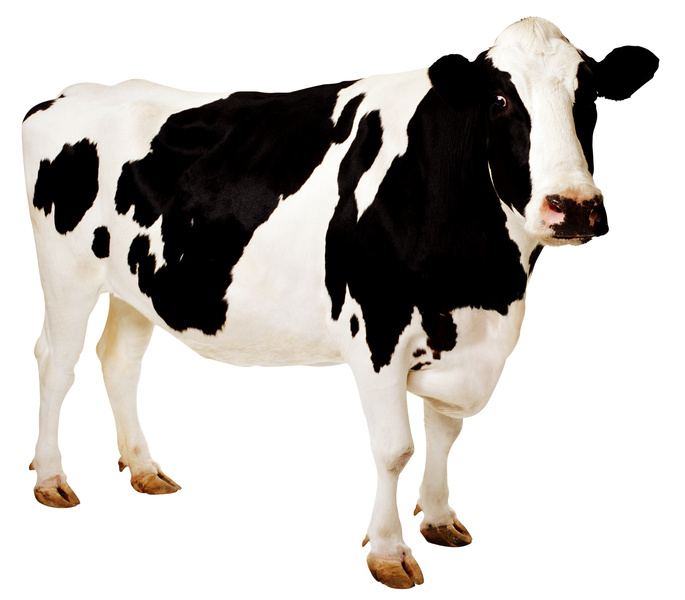
\includegraphics[width=0.1\textwidth]{2010-11-1_700cow} & $\xleftrightarrow{\hspace{0.3\textwidth}}$ & 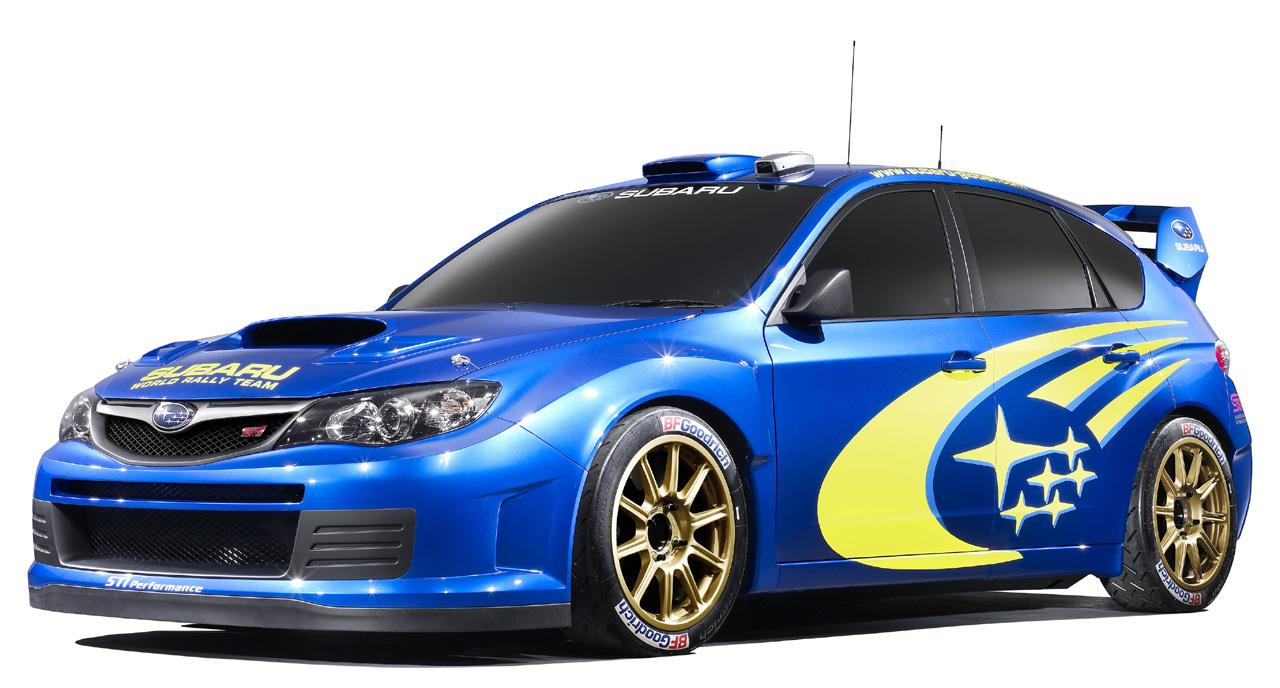
\includegraphics[width=0.1\textwidth]{2010-11-1_2008-subaru-wrc-concept-car1} \\
        \includegraphics[width=0.1\textwidth]{2010-11-1_plane} & $\xleftrightarrow{\hspace{0.3\textwidth}}$ & 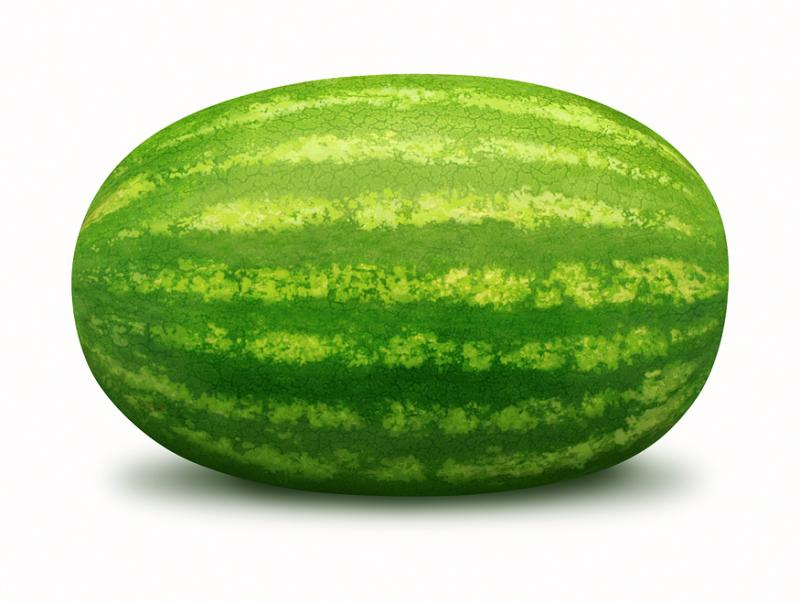
\includegraphics[width=0.1\textwidth]{2010-11-01_watermelon-854} \\
        \includegraphics[width=0.1\textwidth]{2010-11-01_earth-day-action} & $\xleftrightarrow{\hspace{0.3\textwidth}}$ & 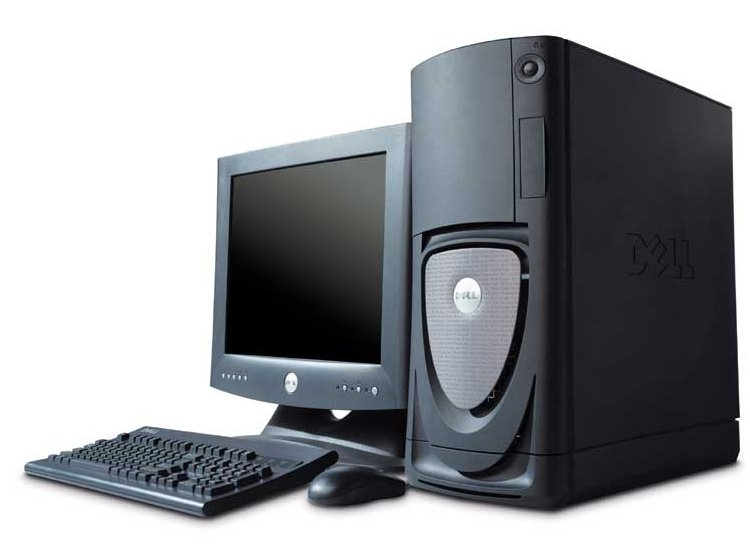
\includegraphics[width=0.1\textwidth]{2010-11-01_DellComputer}
      \end{tabular}
    \end{center}
    \caption{Example pairing showing that $3 = 3$.}\label{fig:3=3}
  \end{figure}

  You might think it obvious, then, that the number of paths our person can walk is bigger than the number of tiles.  We can match each tile with the path that starts on a tile the same color as it, and changes to the other color after it hits this tile.  For example, we would match the third red tile with the path
  \begin{center}
    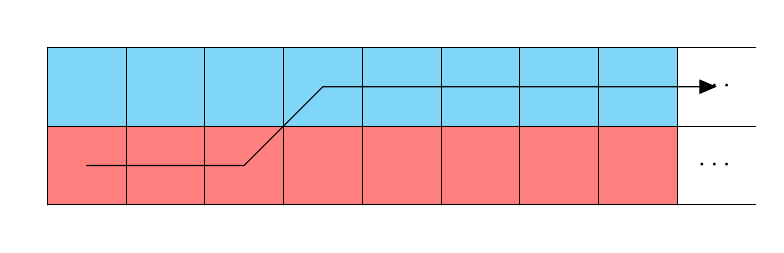
\begin{tikzpicture}[line cap=round,line join=round,>=triangle 45,x=1.0cm,y=1.0cm]
      \clip(-0.25,-1.25) rectangle (9,1.25);
      \foreach \x in {0,1,2,3,4,5,6,7}{
        \fill[cyan,opacity=0.5] (\x,1) -- (\x+1,1) -- (\x+1,0) -- (\x,0) -- cycle;
        \fill[red,opacity=0.5] (\x,-1) -- (\x+1,-1) -- (\x+1,0) -- (\x,0) -- cycle;
%         \foreach \y in {1,-1}{
%           \fill[white] (0.32+\x,0.68*\y) -- (0.68+\x,0.68*\y) -- (0.68+\x,0.32*\y) -- (0.32+\x,0.32*\y) -- cycle;
%         }
        \draw (\x,1)-- (\x,-1);
      }
      \draw (8,1)-- (8,-1);

      \draw (8.5,0.5) node[anchor=center] {$\cdots$};
      \draw (8.5,-0.5) node[anchor=center] {$\cdots$};

      \draw (0,1) -- (9,1);
      \draw (0,0) -- (9,0);
      \draw[-,color=black] (0,-1) -- (9,-1);
      \draw[->] (0.5,-0.5) -- (2.5,-0.5) --
                (3.5,0.5) -- (8.5,0.5);
    \end{tikzpicture}
  \end{center}

  It is important to note, however, that it is not sufficient that we find some matching that leaves things left over.  We must show that \emph{every} matching leaves things left over.  For example, an infinite sidewalk that is one tile across has just as many tiles as an infinite sidewalk that is two tiles across, as we can see from the picture below by matching the 1R on top with the 1R on bottom, the 1B on top with the 1B on bottom, the 2R on top with the 2R on bottom, and so on.

  \begin{center}
    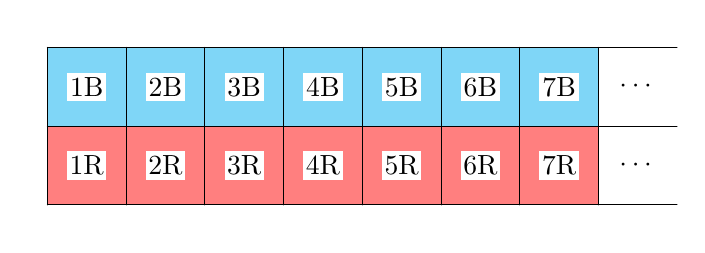
\begin{tikzpicture}[line cap=round,line join=round,>=triangle 45,x=1.0cm,y=1.0cm]
      \clip(-0.25,-1.25) rectangle (8,1.25);
      \foreach \x in {1,2,3,4,5,6,7}{
        \fill[cyan,opacity=0.5] (\x-1,1) -- (\x,1) -- (\x,0) -- (\x-1,0) -- cycle;
        \fill[red,opacity=0.5] (\x-1,-1) -- (\x,-1) -- (\x,0) -- (\x-1,0) -- cycle;
        \foreach \y in {1,-1}{
          \fill[white] (0.25+\x-1,0.68*\y) -- (0.75+\x-1,0.68*\y) -- (0.75+\x-1,0.32*\y) -- (0.25+\x-1,0.32*\y) -- cycle;
        }
        \draw[color=black] (-0.5+\x,0.5) node[anchor=center] {\x B};
        \draw[color=black] (-0.5+\x,-0.5) node[anchor=center] {\x R};
        \draw (\x-1,1)-- (\x-1,-1);
      }
      \draw (7,1)-- (7,-1);

      \draw (7.5,0.5) node[anchor=center] {$\cdots$};
      \draw (7.5,-0.5) node[anchor=center] {$\cdots$};

      \draw (0,1) -- (9,1);
      \draw (0,0) -- (9,0);
      \draw (0,-1) -- (9,-1);
    \end{tikzpicture} \\
    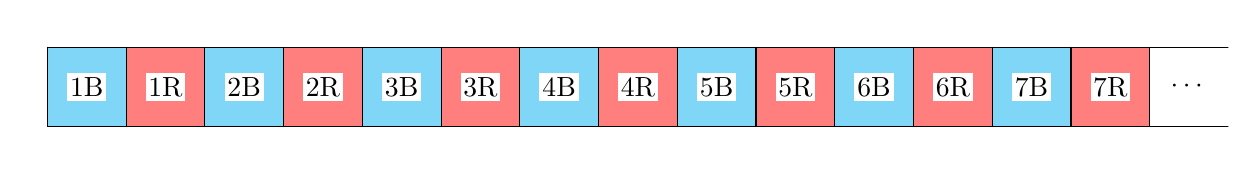
\begin{tikzpicture}[line cap=round,line join=round,>=triangle 45,x=1.0cm,y=1.0cm]
      \clip(0.75,-0.25) rectangle (16,1.25);
      \foreach \x in {1,2,3,4,5,6,7}{
        \fill[cyan,opacity=0.5] (2*\x-1,1) -- (2*\x,1) -- (2*\x,0) -- (2*\x-1,0) -- cycle;
        \fill[red,opacity=0.5] (2*\x,1) -- (2*\x+1,1) -- (2*\x+1,0) -- (2*\x,0) -- cycle;
        \fill[white] (0.25+2*\x-1,0.68) -- (0.75+2*\x-1,0.68) -- (0.75+2*\x-1,0.32) -- (0.25+2*\x-1,0.32) -- cycle;
        \fill[white] (0.25+2*\x,0.68) -- (0.75+2*\x,0.68) -- (0.75+2*\x,0.32) -- (0.25+2*\x,0.32) -- cycle;
        \draw[color=black] (0.5+2*\x-1,0.5) node[anchor=center] {\x B};
        \draw[color=black] (0.5+2*\x,0.5) node[anchor=center] {\x R};
        \draw (2*\x-1,1)-- (2*\x-1,0);
        \draw (2*\x,1)-- (2*\x,0);
      }
      \draw (15,1)-- (15,0);

      \draw (15.5,0.5) node[anchor=center] {$\cdots$};

      \draw (1,1) -- (16,1);
      \draw (1,0) -- (16,0);
    \end{tikzpicture}
  \end{center}

  In fact, if we were only to require that \emph{some} matching leave extra tiles, then the number of tiles in a sidewalk that is one tile wide would not be equal to itself, for we could match the first tile with 1B (in the bottom picture above), the second tile with 2B, and so on, and we would leave over half the tiles!

  In fact, even if we had a \emph{field} of tiles that is infinite in every direction, we would still have no more tiles than if we had only a sidewalk that is one tile across.  The following matching shows this:

  \begin{center}
    \begin{tikzpicture}[line cap=round,line join=round,>=triangle 45,x=1.0cm,y=1.0cm]
      \clip(0.75,-0.25-2.5) rectangle (10,1.25+2.5);
      \foreach \x in {1,2,3,4,5,6,7,8}{
        \draw[color=black] (0.5+\x,0.5) node[anchor=center] {\x};
        \draw (\x,1)-- (\x,0);
      }
      \draw (9,1)-- (9,0);

      \draw (9.5,0.5) node[anchor=center] {$\cdots$};

      \draw (1,1) -- (10,1);
      \draw (1,0) -- (10,0);
    \end{tikzpicture}\quad
    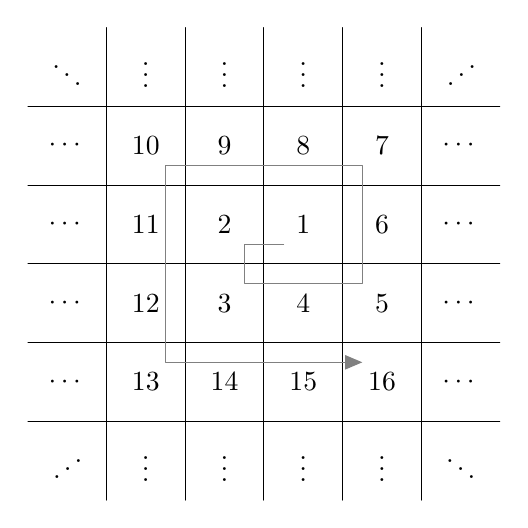
\begin{tikzpicture}[line cap=round,line join=round,>=triangle 45,x=1.0cm,y=1.0cm]
      \clip(-3,-3) rectangle (3,3);
      \foreach \x in {-2,-1,0,1,2}{
        \draw (-3,\x) -- (3,\x);
        \draw (\x,-3) -- (\x,3);
      }
      \foreach \x in {-2,-1,0,1}{
        \draw (-2.5,\x+0.5) node[anchor=center] {$\cdots$};
        \draw (2.5,\x+0.5) node[anchor=center] {$\cdots$};
        \draw (\x+0.5,-2.5) node[anchor=center] {$\vdots$};
        \draw (\x+0.5,2.5) node[anchor=center] {$\vdots$};
      }
      \draw (2.5,2.5) node[anchor=center] {$\iddots$};
      \draw (-2.5,-2.5) node[anchor=center] {$\iddots$};
      \draw (2.5,-2.5) node[anchor=center] {$\ddots$};
      \draw (-2.5,2.5) node[anchor=center] {$\ddots$};

      \draw [->,color=gray] (0.25,0.25) -- (-0.25,0.25) -- (-0.25,-0.25) -- (0.25,-0.25) -- (1.25,-0.25) -- (1.25,0.25) -- (1.25,1.25) -- (0.25,1.25) -- (-0.25,1.25) -- (-1.25,1.25) -- (-1.25,0.25) -- (-1.25,-0.25) -- (-1.25,-1.25) -- (-0.25,-1.25) -- (0.25,-1.25) -- (1.25,-1.25);
      \draw (0.5,0.5) node[anchor=center] {1};
      \draw (-0.5,0.5) node[anchor=center] {2};
      \draw (-0.5,-0.5) node[anchor=center] {3};
      \draw (0.5,-0.5) node[anchor=center] {4};
      \draw (1.5,-0.5) node[anchor=center] {5};
      \draw (1.5,0.5) node[anchor=center] {6};
      \draw (1.5,1.5) node[anchor=center] {7};
      \draw (0.5,1.5) node[anchor=center] {8};
      \draw (-0.5,1.5) node[anchor=center] {9};
      \draw (-1.5,1.5) node[anchor=center] {10};
      \draw (-1.5,0.5) node[anchor=center] {11};
      \draw (-1.5,-0.5) node[anchor=center] {12};
      \draw (-1.5,-1.5) node[anchor=center] {13};
      \draw (-0.5,-1.5) node[anchor=center] {14};
      \draw (0.5,-1.5) node[anchor=center] {15};
      \draw (1.5,-1.5) node[anchor=center] {16};
    \end{tikzpicture}
  \end{center}

  You might wonder, given that there are so many different ways to match up infinitely many things, how we can know that there is no matching that catches everything.  I will now prove that, no matter how you try to match paths (ways of walking) and tiles, you will miss some tiles.  Since we have already seen that the number of tiles in a sidewalk two tiles wide is the same as the number of tiles in a sidewalk one tile wide, I will show that any matching between paths and tiles in a sidewalk one tile wide misses some paths.  I will do this by creating a path that does not match the path we have chosen for any tile.

  \makeatletter
  \newcommand{\tile}[1]{
    \begingroup
      \newcount\@n
      \@n=1\relax
      \loop
        \framebox[2\height][c]{\the\@n}\hspace{-\fboxrule}%
      \ifnum\@n<#1\relax\advance\@n by 1\repeat
      \let\@vrule=\vrule
      \renewcommand{\vrule}[6]{\phantom{\@vrule##1##2##3##4##5##6}}% this is a terrible hack, and relies on the fact that the command I'm patching uses ``\vrule \@width \fboxrule \@height \dimen@ \@depth \z@'' and doesn't explicitly put in arguments.  Grrr TeX code that doesn't patch well.
      \framebox[2\height][c]{{\let\vrule\@vrule\ \vphantom{1}\small$\cdots$}}% \small requires a functional \vrule!?
    \endgroup
  }
  \makeatother
  
  Suppose we are given a matching between tiles and paths.  Since we have numbered the tiles in a sidewalk one tile wide (\tile{8}), we also have a numbering of the paths in our matching.  Consider a new path that differs from the $n^\text{th}$ path in our matching on the $n^\text{th}$ tile, that is, the $n^\text{th}$ step that you take.  For example, if our first eight paths are
  \newcommand{\sidewalk}[2][-1]{
    \tiny
    \begin{tikzpicture}[line cap=round,line join=round,>=triangle 45,x=0.5cm,y=0.5cm]
      \clip(-0.25,-1.25) rectangle (9,1.25);
      \def\highlight{}
      \foreach \x in {0,1,2,3,4,5,6,7}{
        \fill[cyan,opacity=0.5] (\x,1) -- (\x+1,1) -- (\x+1,0) -- (\x,0) -- cycle;
        \fill[red,opacity=0.5] (\x,-1) -- (\x+1,-1) -- (\x+1,0) -- (\x,0) -- cycle;
        \ifnum\x=\numexpr#1-1\relax
          \xdef\highlight{\noexpand\draw[yellow,very thick] (\x,1) -- (\x+1,1) -- (\x+1,-1) -- (\x,-1) -- cycle;}
        \fi
%         \foreach \y in {1,-1}{
%           \fill[white] (0.32+\x,0.68*\y) -- (0.68+\x,0.68*\y) -- (0.68+\x,0.32*\y) -- (0.32+\x,0.32*\y) -- cycle;
%         }
        \draw (\x,1)-- (\x,-1);
      }
      \draw (8,1)-- (8,-1);

      \draw (8.5,0.5) node[anchor=center] {$\cdots$};
      \draw (8.5,-0.5) node[anchor=center] {$\cdots$};

      \draw (0,1) -- (9,1);
      \draw (0,0) -- (9,0);
      \draw (0,-1) -- (9,-1);
      \highlight
      #2
    \end{tikzpicture}
  }
  \begin{center}
    \newsavebox{\sidewalkbox}
    \savebox{\sidewalkbox}{\sidewalk{}}
    \newlength{\sidewalkwidth}
    \setlength{\sidewalkwidth}{\widthof{\usebox{\sidewalkbox}}}
    \huge
% StringJoin["\\draw[->] ",
%    Table[StringJoin["(", ToString[#[[i]][[1]]], ",",
%       ToString[#[[i]][[2]]], ") -- "], {i, 1, Length[#]}] /.
%     List -> StringJoin, "(8.5,",
%    ToString[#[[Length[#]]][[2]]/2 +
%      0.25 (2 RandomInteger[{0, 1}] - 1)], ");"] &[
%  Table[{x + 0.5, (2 RandomInteger[{0, 1}] - 1) 0.5}, {x, 0, 6}]]
     \begin{tabular}{m{\widthof{1:}}@{}m{\sidewalkwidth}m{\widthof{1:}}@{}m{\sidewalkwidth}}
       1: &
        \sidewalk[1]{
          \draw[->] (0.5,0.5) -- (1.5,-0.5) --
                    (2.5,0.5) -- (3.5,-0.5) --
                    (4.5,0.5) -- (5.5,-0.5) --
                    (6.5,0.5) -- (7.5,-0.5) --
                    (8.5,0.5) -- (9,0);
        } &
      2: &
        \sidewalk[2]{\draw[->] (0.5,0.5) -- (8.5,0.5);} \\
      3: &
        \sidewalk[3]{\draw[->] (0.5,-0.5) -- (8.5,-0.5);} &
      4: &
        \sidewalk[4]{\draw[->] (0.5,0.5) -- (1.5,-0.5) -- (2.5,-0.5) -- (3.5,-0.5) -- (4.5,-0.5) -- (5.5,-0.5) -- (6.5,0.5) -- (7.5,0.5) -- (8.5,0.5);} \\
      5: &
        \sidewalk[5]{\draw[->] (0.5,-0.5) -- (1.5,0.5) -- (2.5,0.5) -- (3.5,-0.5) -- (4.5,0.5) -- (5.5,-0.5) -- (6.5,-0.5) -- (7.5,0.5) -- (8.5,-0.5);} &
      6: &
        \sidewalk[6]{\draw[->] (0.5,-0.5) -- (1.5,0.5) -- (2.5,-0.5) -- (3.5,-0.5) -- (4.5,0.5) -- (5.5,0.5) -- (6.5,-0.5) -- (7.5,-0.5) -- (8.5,-0.5);} \\
      7: &
        \sidewalk[7]{\draw[->] (0.5,0.5) -- (1.5,-0.5) -- (2.5,-0.5) -- (3.5,-0.5) -- (4.5,-0.5) -- (5.5,-0.5) -- (6.5,-0.5) -- (7.5,0.5) -- (8.5,-0.5);} &
      8: &
        \sidewalk[8]{\draw[->] (0.5,0.5) -- (1.5,-0.5) -- (2.5,-0.5) -- (3.5,0.5) -- (4.5,0.5) -- (5.5,0.5) -- (6.5,0.5) -- (7.5,0.5) -- (8.5,-0.5);}
     \end{tabular}
  \end{center}
  \noindent then our new path is
  \begin{center}
    \sidewalk{\draw[->] (0.5,-0.5) -- (1.5,-0.5) -- (2.5,0.5) -- (3.5,0.5) -- (4.5,-0.5) -- (5.5,-0.5) -- (6.5,0.5) -- (7.5,-0.5) -- (8.5,-0.5);}
  \end{center}

  Clearly, this path is not any of the ones in the matching, because it differs from every single path on at some point (in particular, it differs from the $n^\text{th}$ path on the $n^\text{th}$ tile, the $n^\text{th}$ step you take, which is highlighted in yellow).
  
  Thus, we see that the number of paths a person can take is strictly larger than the number of tiles in the sidewalk.


\clearpage
\section{Audience: Adult}
  Recall that real numbers are numbers with a decimal expansion, for example 1, 2, $3.5$, $\pi = 3.14159265$\ldots  Every real number has an infinite decimal expansion, for example $1 = 1.0000000000$\ldots, $2 = 2.0000000000$\ldots, $3.5 = 3.5000000000$\ldots  Recall that the rational numbers are fractions of integers, for example $1 = \frac11$, $\frac32$, $\frac{100}{101}$, $\frac{22}{7}$.  The positive integers are the integers greater than zero, 1, 2, 3, 4, \ldots  There is a theorem in math that states that the rational numbers are \emph{countable}, that is, that the set of rational numbers is the same size as the set of positive integers, and another theorem which states that the real numbers are \emph{uncountable}, that is, that the set of real numbers is strictly bigger.  By this (``same size'' and ``strictly bigger'') I mean that it is possible to match every rational number with some positive integer in a way so that there are no rational numbers, nor positive integers, left unmatched, but that any matching you make between real numbers and positive integers leaves some real numbers not matched with anything. 
  
  If you imagine laying the rational numbers out on a two-dimensional grid, so that the number $p / q$ falls at $(p, q)$, then we may match the positive integers with the rational numbers by walking in a spiral pattern out from zero, skipping over numbers that we have already counted (or that are undefined, such as zero divided by any number).  The beginning of this sequence is $\frac01$, $\frac11$, $\frac12$, $\frac{-1}{2}$, $\frac{-1}{1}$, \ldots  Graphically, this is:
  \begin{center}
    \makeatletter
    \newcount\m
    \newcount\n
    \newcount\q
    \newcount\r
    \def\fullexpand#1{{\edef\@temp{#1}\expandafter}\@temp}
    %
    \newcommand{\@gcd}[2]{{%
      \m=#1 \n=#2
      %\m = \q\n + \r
      \ifnum\m=0
        \ifnum\n=0
          \expandafter\xdef\csname gcd\the\m, \the\n\endcsname{\infty}%(0, 0) = \infty
        \else
          \expandafter\xdef\csname gcd\the\m, \the\n\endcsname{\the\n}% (0, n) = n
        \fi
      \else
        \ifnum\n=0
          \expandafter\xdef\csname gcd\the\m, \the\n\endcsname{\the\m}% (m, 0) = m
        \else
          \ifnum\m<0
            \ifnum\n<0
              \@gcd{-\the\m}{-\the\n}%
              \expandafter\xdef\csname gcd\the\m, \the\n\endcsname{-\csname gcd\expandafter\@gobble\the\m, \expandafter\@gobble\the\n\endcsname}% remember gcd(n, m)
            \else
              \@gcd{-\the\m}{\the\n}%
              \expandafter\xdef\csname gcd\the\m, \the\n\endcsname{\csname gcd\expandafter\@gobble\the\m, \the\n\endcsname}% remember gcd(n, m)
            \fi
          \else
            \ifnum\n<0
              \@gcd{\the\m}{-\the\n}%
              \expandafter\xdef\csname gcd\the\m, \the\n\endcsname{-\csname gcd\the\m, \expandafter\@gobble\the\n\endcsname}% remember gcd(n, m)
            \else
              \q = \m  \divide\q by \n % calculate \q = m / n
              \r = \q  \multiply\r by -\n \advance\r by \m % calculate \r = -\q\n + \m
              \@gcd{\the\n}{\the\r}% recurse
              \expandafter\xdef\csname gcd\the\m, \the\n\endcsname{\csname gcd\the\n, \the\r\endcsname}% remember gcd(n, m)
              %\global\expandafter\let\csname gcd\the\n, \the\r\endcsname=\relax % forget gcd(n, r)
            \fi
          \fi
        \fi
      \fi
    }}
    \newcommand{\ifgcdone}[2]{%
      {\@gcd{#1}{#2}\expandafter}%
      \ifnum\csname gcd#1, #2\endcsname=1
        \expandafter\@firstoftwo
      \else
        \expandafter\@secondoftwo
      \fi
    }
    \makeatother
    \def\arrowcolor{green}
    \def\arrowoffset{0.33}
    \begin{tikzpicture}[line cap=round,line join=round,>=triangle 45,x=1cm,y=1cm]
      %\draw[->,color=black] (-3.5,0) -- (3.5,0);
      %\foreach \x in {-3,-2,-1,1,2,3}
      %\draw[shift={(\x,0)},color=black] (0pt,2pt) -- (0pt,-2pt) node[below] {\footnotesize $\x$};
      %\draw[->,color=black] (0,-3.86) -- (0,6.3);
      %\foreach \y in {-3,-2,-1,1,2,3,4,5,6}
      %\draw[shift={(0,\y)},color=black] (2pt,0pt) -- (-2pt,0pt) node[left] {\footnotesize $\y$};
      %\draw[color=black] (0pt,-10pt) node[right] {\footnotesize $0$};
      %\clip(-4.3,-3.86) rectangle (8.26,6.3);
      \clip(-3.5,-3.5) rectangle (3.5,3.5);
      \foreach \x in {-3,-2,-1,0,1,2,3}{
        \foreach \y in {-3,-2,-1,0,1,2,3}{
          \ifnum\y=0
            \draw[color=gray] (\x,\y) node[anchor=center] {$\frac{\x}{\y}$};
            \draw (\x,\y) node[anchor=center] {$/$};
            \draw (\x,\y) node[anchor=center] {$\backslash$};
          \else
            \ifgcdone{\x}{\y}{%
              \draw
            }{%
              \draw[color=gray]
            } (\x,\y) node[anchor=center] {$\frac{\x}{\y}$};
          \fi
        }
      }
      \draw[color=\arrowcolor] (0.8*\arrowoffset,1-0.8*\arrowoffset) -- (0.8*\arrowoffset,1+0.8*\arrowoffset) -- (-0.8*\arrowoffset,1+0.8*\arrowoffset) -- (-0.8*\arrowoffset,1-0.8*\arrowoffset) -- cycle;
      \draw[->,color=\arrowcolor] (\arrowoffset,1) -- (1-\arrowoffset,1);
      \draw[->,color=\arrowcolor] (1,1+\arrowoffset) -- (1,2-\arrowoffset);
      \draw[->,color=\arrowcolor] (1-\arrowoffset,2) -- (-1+\arrowoffset,2);
      \draw[->,color=\arrowcolor] (-1,2-\arrowoffset) -- (-1,1+\arrowoffset);
      \draw[->,color=\arrowcolor] (-1,1-\arrowoffset) -- (2,1-\arrowoffset);
      \draw[->,color=\arrowcolor] (2,1+\arrowoffset) -- (2,3-\arrowoffset);
      \draw[->,color=\arrowcolor] (2-\arrowoffset,3) -- (1+\arrowoffset,3);
      \draw[->,color=\arrowcolor] (1-\arrowoffset,3) -- (-1+\arrowoffset,3);
      \draw[->,color=\arrowcolor] (-1-\arrowoffset,3) -- (-2+\arrowoffset,3);
      \draw[->,color=\arrowcolor] (-2,3-\arrowoffset) -- (-2,1+\arrowoffset);
      \draw[->,color=\arrowcolor] (-2,1-1.5*\arrowoffset) -- (3,1-1.5*\arrowoffset);
      \draw[->,color=\arrowcolor] (3,1+\arrowoffset) -- (3,2-\arrowoffset);
    \end{tikzpicture}
  \end{center}
  \noindent This shows that the rational numbers are countable.
  
  The real numbers, however, cannot be matched with the positive integers.  I show this by contradiction; I show that if there is such a matching, then we can conclude nonsensical statements (and if making a new assumption allows us to conclude nonsense, then the assumption itself must be nonsense).  Suppose we have such a matching.  We can construct a new real number that differs in its $n^\text{th}$ decimal digit from the real number matched with $n$.  For example, if we were given a matching that matched 1 with $1.8$, 2 with $1.26$, 3 with $5.758$, 4 with $1$, and 5 with $\pi$, then our new number could be $0.11111$, which differs from $1.8$ in the first decimal place (the $0.1$ place), $1.26$ in the second decimal place (the $0.01$ place), and so on.  It is clear that this number cannot be matched with any number under the matching we are given, because, if it were matched with $n$, then it would differ from itself in the $n^\text{th}$ decimal digit, which is nonsense.  Thus, there is no matching between the real numbers and the positive integers.

\clearpage
\section{Audience: Mathematician}
  I will prove that the rational numbers are countable, and present a variant of Cantor's diagonalization argument to prove the real numbers are uncountable.  This constructively proves that there exist uncountable sets (the real numbers are such an example). % Additionally, in measure theory, the fact that the real numbers are uncountable allows us to say that all countable sets are relatively tiny (have measure zero) as subsets of the reals.
  \begin{defn*}
    The set of \emph{rational numbers}, $\mathbb Q$, is the set of integer fractions $\frac{p}{q}$ in reduced form; the greatest common divisor of $p$ and $q$ is one.
    %The \emph{rational numbers} are the set $$\mathbb Q \defeq \left.\mathset[(a, b)]{a,b\in\mathbb Z\text{ and }b> 0} \right/\sim$$
    %where
    %$$(a, b) \sim (c, d)\qquad\text{whenever }ad - bc = 0.$$
    %The congruence class $\overline{(a, b)} \in \mathbb Q$ is denoted $a / b$ or $\frac{a}{b}$.  Note that this denotation is not unique.
  \end{defn*}
  \begin{defn*}
    The \emph{counting numbers} are the set $$\mathbb N \defeq \{1, 2, 3, 4, 5, 6, 7, 8, 9, 10, \ldots\}.$$
  \end{defn*}
  \begin{defn*}
    A set $S$ is \emph{countable} if there is some surjection from the counting numbers onto $S$.
  \end{defn*}
  \begin{defn*}
    A set $S$ is \emph{uncountable} if it is not countable.
  \end{defn*}
  \begin{thm*}
    The rational numbers are countable.
  \end{thm*}
  The proof is, essentially, that $\mathbb N \times \mathbb N$ is isomorphic to $\mathbb N$; we count in a roughly spiral pattern centered at zero.
  \begin{proof}
    Define the \emph{height} of $\frac{a}{b}$ to be $|a| + |b|$.  We may count the rational numbers in order of height, and ordering by $a$, and then $b$, when the heights are the same.  The beginning of this counting is $0 / 1$, $-1 / 1$, $1 / 1$, $-2 / 1$, $-1 / 2$, $1 / 2$, $2 / 1$, \ldots  Since there are at most $(2d+1)^2$ rational numbers of height less than or equal to $d$, a rational number with height $d$ is mapped on to by one of the counting numbers up to $(2d+1)^2$; every rational number is mapped onto by this counting.  Thus, the rational numbers are countable.
  \end{proof}
  \noindent \textsc{Note}: It is not hard to extend this proof to show that $\mathbb N^n$ is countable for any finite $n$.
  
  I use the decimal representation of the real numbers to prove the following theorem.  I use an overline ( $\bar{}$ ) to mean that the digit(s) under it are repeated forever.  Note that $a.bcd\cdots z\overline{9} = a.bcd\cdots (z+1)\overline{0}$ (if $z < 9$; otherwise, we need to continue carrying the one); $\sum_{i=k}^\infty 10^{-k} \cdot 9 = 1 \cdot 10^{-k + 1} + \sum_{i=k}^\infty 10^{-k} \cdot 0$.  Furthermore, these are the only equivalences between decimal representations; there are no other real numbers with multiple representations, and these real numbers have only these two decimal representations.
  \begin{thm*}
    The real numbers are uncountable.
  \end{thm*}
  \begin{proof}
    Suppose, for contradiction, that the real numbers are countable; suppose that $f: \mathbb N \twoheadrightarrow \mathbb R$ is a surjection.  Let $r_n$ denote the $n^\text{th}$ decimal digit of $r$, so that the fractional part of $r$ is $r_1r_2r_3r_4r_5$\ldots  Then define a real number $r'$ with $0 \le r' < 1$ so that $r'_n$ is 5 if $(f(n))_n \ne 5$, and 6 if $(f(n))_n = 5$.  Then there can be no $n$ such that $r' = f(n)$ since $r'_n \ne (f(n))_n$.  Thus $f$ is not surjective, contradicting our assumption, and $\mathbb R$ is uncountable.
  \end{proof}
  Note that choosing 5 and 6 as our allowable digits for $r'$ side-steps the issue that $0.\overline{9} = 1.\overline{0}$.  


\end{document}

